\documentclass[12pt,english,dvipsnames,aspectratio=169,handout]{beamer}\usepackage[]{graphicx}\usepackage[]{xcolor}
% maxwidth is the original width if it is less than linewidth
% otherwise use linewidth (to make sure the graphics do not exceed the margin)
\makeatletter
\def\maxwidth{ %
  \ifdim\Gin@nat@width>\linewidth
    \linewidth
  \else
    \Gin@nat@width
  \fi
}
\makeatother

\definecolor{fgcolor}{rgb}{0.345, 0.345, 0.345}
\newcommand{\hlnum}[1]{\textcolor[rgb]{0.686,0.059,0.569}{#1}}%
\newcommand{\hlstr}[1]{\textcolor[rgb]{0.192,0.494,0.8}{#1}}%
\newcommand{\hlcom}[1]{\textcolor[rgb]{0.678,0.584,0.686}{\textit{#1}}}%
\newcommand{\hlopt}[1]{\textcolor[rgb]{0,0,0}{#1}}%
\newcommand{\hlstd}[1]{\textcolor[rgb]{0.345,0.345,0.345}{#1}}%
\newcommand{\hlkwa}[1]{\textcolor[rgb]{0.161,0.373,0.58}{\textbf{#1}}}%
\newcommand{\hlkwb}[1]{\textcolor[rgb]{0.69,0.353,0.396}{#1}}%
\newcommand{\hlkwc}[1]{\textcolor[rgb]{0.333,0.667,0.333}{#1}}%
\newcommand{\hlkwd}[1]{\textcolor[rgb]{0.737,0.353,0.396}{\textbf{#1}}}%
\let\hlipl\hlkwb

\usepackage{framed}
\makeatletter
\newenvironment{kframe}{%
 \def\at@end@of@kframe{}%
 \ifinner\ifhmode%
  \def\at@end@of@kframe{\end{minipage}}%
  \begin{minipage}{\columnwidth}%
 \fi\fi%
 \def\FrameCommand##1{\hskip\@totalleftmargin \hskip-\fboxsep
 \colorbox{shadecolor}{##1}\hskip-\fboxsep
     % There is no \\@totalrightmargin, so:
     \hskip-\linewidth \hskip-\@totalleftmargin \hskip\columnwidth}%
 \MakeFramed {\advance\hsize-\width
   \@totalleftmargin\z@ \linewidth\hsize
   \@setminipage}}%
 {\par\unskip\endMakeFramed%
 \at@end@of@kframe}
\makeatother

\definecolor{shadecolor}{rgb}{.97, .97, .97}
\definecolor{messagecolor}{rgb}{0, 0, 0}
\definecolor{warningcolor}{rgb}{1, 0, 1}
\definecolor{errorcolor}{rgb}{1, 0, 0}
\newenvironment{knitrout}{}{} % an empty environment to be redefined in TeX

\usepackage{alltt}
\usepackage{fontspec}
\setsansfont[Mapping=tex-text]{Fira Sans}
\setcounter{secnumdepth}{4}
\setcounter{tocdepth}{4}
\usepackage[normalem]{ulem}
\usepackage[T1]{fontenc}
\usepackage{dcolumn}
\usepackage{booktabs}
\usepackage{bm}
\usepackage{setspace}
\makeatletter
\usetheme{metropolis}
\setbeamertemplate{frame footer}{Bosancianu | Schaub | Hertie School}
\setbeamerfont{page number in head/foot}{size=\tiny}
\setbeamercolor{footline}{fg=gray}
\usepackage{xcolor}
\setbeamercovered{dynamic}
\usepackage{tikz}
\usetikzlibrary{arrows, positioning,fit,shapes.misc}
\usepackage[labelformat=empty]{caption}
% For table captions in Beamer
\usepackage[sectionbib]{apacite}
\renewcommand{\bibliographytypesize}{\footnotesize}
\makeatletter
\let\st@rtbibsection\@bibnewpage
\let\st@rtbibchapter\@bibnewpage
\makeatother
\usepackage{amsmath, mathtools}
\usepackage{xunicode}
\usepackage{hyperref}
\graphicspath{{./figures/}} 
% Defines a checkmark
\def\checkmark{\tikz\fill[scale=0.4,color=orange](0,.35) -- (.25,0) -- (1,.7) -- (.25,.15) -- cycle;}
\newcommand{\indep}{\perp \!\!\!\! \perp}
\setbeamertemplate{itemize items}{\checkmark}
\usepackage{multirow}
\hypersetup{pdfauthor={Bosancianu and Schaub},
	pdftitle={Statistical Modeling and Causal Inference with R},
	pdfsubject={Week 7: Regression Discontinuity Designs},
	pdfkeywords={Berlin, Hertie, 2020, week 7, RDD}}
\title{\textsc{Statistical Modeling and Causal Inference with R}}
\subtitle{Week 7: Regression Discontinuity Designs}
\date{October 26, 2020}
\author{Manuel Bosancianu \hfill Max Schaub}
\institute{Hertie School of Governance}
\IfFileExists{upquote.sty}{\usepackage{upquote}}{}
\begin{document}
\maketitle




\begin{frame}
	\frametitle{Recap}
	\textcolor{orange}{Matching}: ``plugging in'' the missing potential outcome for each treatment unit by using a control group unit.\bigskip
	\pause
	
	How to choose: a control unit that is ``closest'' to the treatment unit on a set of covariates, $X$.\bigskip
	\pause
	
	Two broad types of matching:
	
	\begin{itemize}
	\item \textcolor{orange}{exact}: looking for identical values on $X$;
	\pause
	\item \textcolor{orange}{approximate}: looking for closest value on $X$.
	\end{itemize}
	
\end{frame}


\begin{frame}
	\frametitle{Recap}
  Sophisticated implementations: propensity scores and coarsened exact matching.\bigskip
  \pause
  
  One major problem is that matching can only address imbalance on \textcolor{orange}{observables}.\bigskip
  
  If there is serious suspicion that unobserved covariates are responsible for imbalances, matching can't help.\bigskip
  \pause
  
  Nothing beats randomization when looking to solve this kind of problem\dots
	
\end{frame}


\begin{frame}
	\frametitle{Today's focus}
	
	\begin{itemize}
		\setlength\itemsep{1.5em}
		\item Core features of the RDD
		\item Sharp RDD
		\item Estimation approaches in Sharp RDD
		\item Diagnostics of an RDD
		\item Example: female empowerment and its political determinants
		\item Fuzzy RDD
	\end{itemize}
\end{frame}


\section{Introduction}

\begin{frame}
\frametitle{RDD: core features}

Introduced in educational studies by \citeA{thistlethwaite_rdd_1960}: rife with examples of cutoffs, tests, and selection procedures.\bigskip
\pause

In economics, analyses only appear at the end of 90s (still dealing with education).\bigskip
\pause

Setup is simple:
\begin{itemize}
\item a score (running/forcing variable, index): a variable which ranks units;
\pause
\item a cutoff: a threshold for the score, which separates units in the treatment and control group;
\pause
\item a treatment: a particular intervention.
\end{itemize}

\end{frame}


\begin{frame}
\frametitle{RDD: core features}

Defining feature: probability of treatment assignment as function of score changes discontinuously at cutoff.\bigskip
\pause



\begin{figure}
\centering
\visible<2->{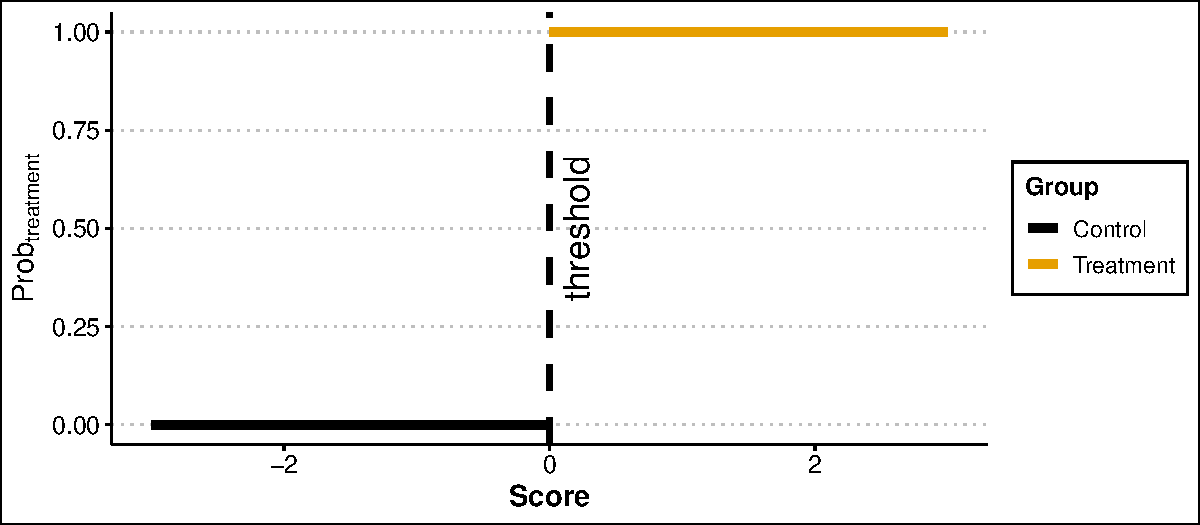
\includegraphics[scale=0.3]{../04-figures/07/01.pdf}}
\visible<2->{\caption{A sharp RD design}}
\end{figure}
\pause

Selection into treatment is non-random, but around the threshold we might benefit from \textit{local randomization}.
\end{frame}


\begin{frame}
\frametitle{RDD: benefits}

\begin{itemize}
\setlength\itemsep{1.5em}
\item analysis relatively accessible to audience \pause
\item assumptions related to score, treatment and cutoff can usually be empirically tested \pause
\item extensive array of falsification tests and validity checks \pause
\item flexibility: time, geography, multiple scores, multiple cutoffs
\end{itemize}

\end{frame}


\section{Empirics I}

\begin{frame}
\frametitle{\citeA{meyersson_islamic_2014} data}

What effect does political control by Islamist parties have on the political empowerment of women?\bigskip
\pause

1994 municipal elections in Turkey: 2 Islamic parties (\textit{Refah} and \textit{B\"{u}y\"{u}k Birlik Partisi}) win the mayorship of 329 municipalities.\bigskip
\pause

Outcomes targeted:

\begin{itemize}
\item educational enrollment of women;
\item adolescent marriages;
\item political participation of women.
\end{itemize}

\end{frame}


\begin{frame}
\frametitle{\citeA{meyersson_islamic_2014} data}






\begin{figure}
\centering
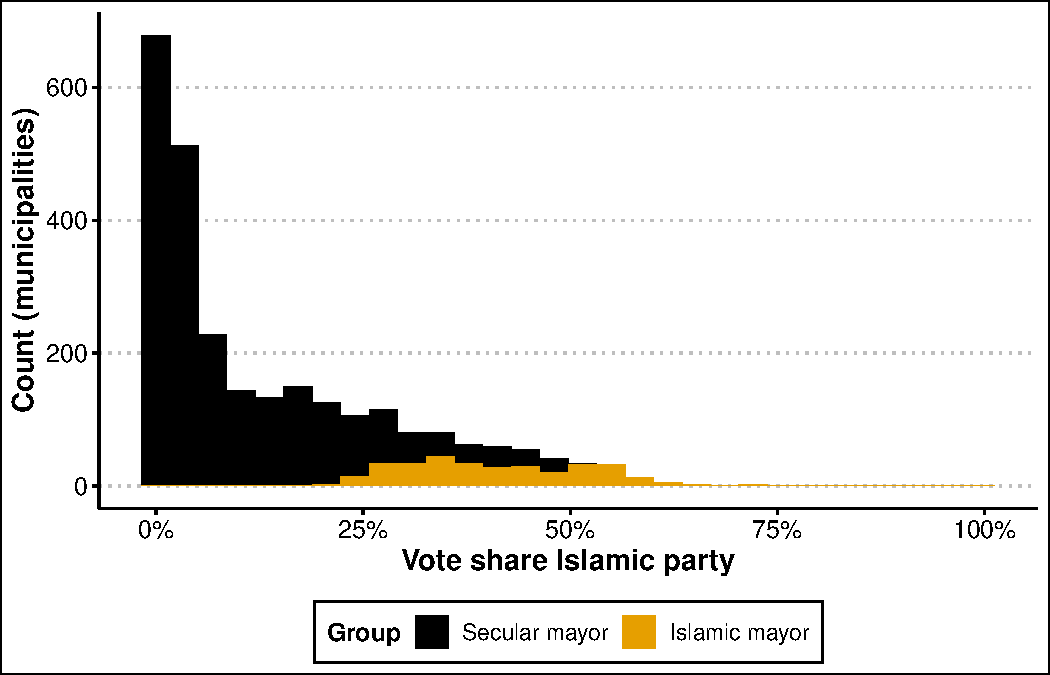
\includegraphics[scale=0.6]{../04-figures/07/02.pdf}
\caption{Distribution of municipalities}
\end{figure}

\end{frame}



\begin{frame}
\frametitle{Women's empowerment}



\begin{figure}
\centering
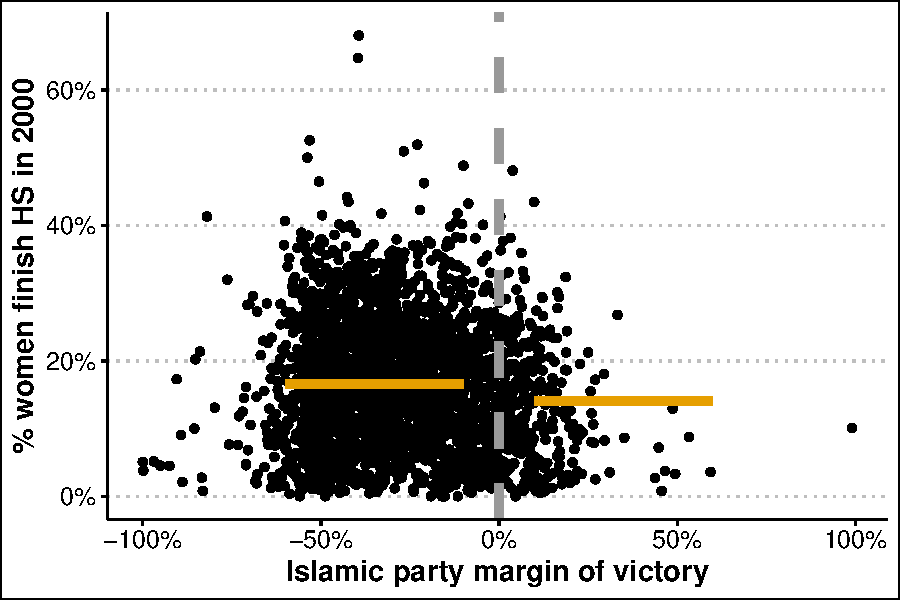
\includegraphics[scale=0.6]{../04-figures/07/03.pdf}
\caption{Association: female education and political power}
\end{figure}

\end{frame}


\begin{frame}
\frametitle{Women's empowerment}
HS completion below cutoff = 0.166152.

HS completion above cutoff = 0.140373.\bigskip
\pause

Many ways in which municipalities where Islamic parties have margin above, say, 5\% are different than the rest.\bigskip
\pause

However, in a short window around the 0\% cutoff, we might benefit from local randomization.

\end{frame}


\section{Sharp RDD}

\begin{frame}
\frametitle{Sharp RDD}
Two broad design types:

\begin{itemize}
\item \textcolor{orange}{sharp}: treatment assigned = treatment received
\item \textcolor{orange}{fuzzy}: compliance with treatment assignment is imperfect
\end{itemize}
\bigskip
\pause

We use experimental language, but ``treatment'' is defined \textit{ex post} by researcher.\bigskip
\pause

Observed outcomes (\textit{c} is cutoff):

\begin{equation}
Y_i = (1 - T_i)*Y_{0i} + T_i*Y_{1i} = \begin{cases}
Y_{0i}, & if\; X_i < c \\
Y_{1i}, & if\; X_i \geq c 
\end{cases}
\end{equation}

\end{frame}


\begin{frame}
\frametitle{Sharp RDD}

\begin{columns}
	\begin{column}{0.55\textwidth}
		Observed expected outcome is:
		
		\begin{equation}
			\footnotesize
			E[Y_i | X_i] = \begin{cases}
				E[Y_{0i} | X_i], & if\; X_i < c \\
				E[Y_{1i} | X_i], & if\; X_i \geq c 
			\end{cases}
		\end{equation}
	\end{column}
	\begin{column}{0.45\textwidth}
		\begin{figure}
			\centering
			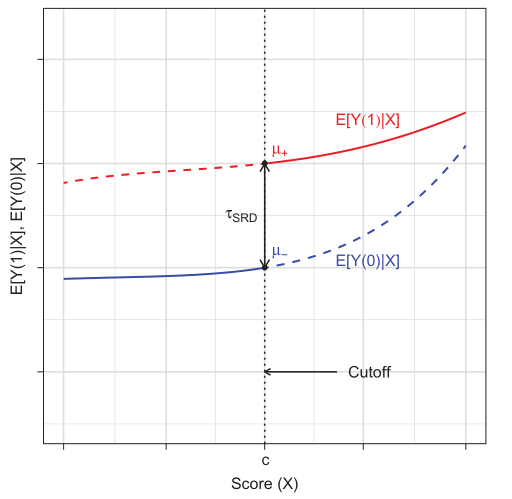
\includegraphics[scale=0.35]{../04-figures/07/04.PNG}
			\caption{Treatment effect in sharp RDD \cite{cattaneo_practical_2019}}
		\end{figure}
	\end{column}
\end{columns}
\pause

RDD relies on extrapolation toward cutoff, to be able to compute $\tau_{SRD}$.

\end{frame}


\begin{frame}
\frametitle{Sharp RDD}

We can't compute $E[Y_{1i} | X_i = x] - E[Y_{0i} | X_i = x]$ for almost any value of $X$.\bigskip
\pause

The cutoff $c$ is the only exception to this (we ``almost'' observe both lines).\bigskip
\pause

\begin{equation}
\tau_{SRD} = E[Y_{1i} | X_i = c] - E[Y_{0i} | X_i = c] \equiv \mu_+ - \mu_-
\end{equation}\bigskip
\pause

Treatment is local in nature (LATE)!

\end{frame}



\begin{frame}
\frametitle{Continuity assumption}
A function $f(x)$ is continuous at the point $x=a$ if $f(x)$ and $f(a)$ get closer to each other as $x$ gets closer to $a$.\bigskip
\pause

If $E[Y_{1i} | X_i = x]$ and $E[Y_{0i} | X_i = x]$ are continuous at $x = c$, then:

\begin{equation}
E[Y_{1i} - Y_{0i} | X_i = c] = \lim_{x \downarrow c}E[Y_i | X_i = x] - \lim_{x \uparrow c}E[Y_i | X_i = x]
\end{equation}
\pause

Conditioning on $X_i$ is impossible (no common support), but extrapolation allows us to compensate for this at $X_i=c$.

\end{frame}



\begin{frame}
\frametitle{Local nature of effects}

We compute the effect, $\tau_{SRD}$, at a single point: $c$.\bigskip
\pause

When treatment effect varies as a function of score $X$, $\tau_{SRD}$ not informative outside of $c$.\pause

\begin{figure}
\centering
\visible<3>{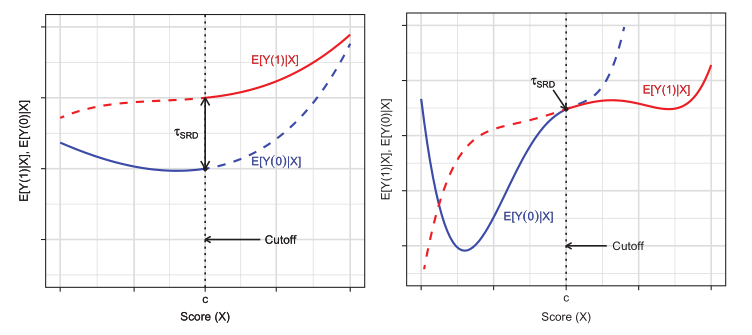
\includegraphics[scale=0.45]{../04-figures/07/05.PNG}}
\visible<3>{\caption{Treatment effect heterogeneity \cite{cattaneo_practical_2019}}}
\end{figure}

\end{frame}


\section{Estimation}

\begin{frame}
\frametitle{Estimating RD effects}
Two strategies:

\begin{itemize}
\setlength\itemsep{1.5em}
\item \textcolor{orange}{continuity-based}: using local polynomial methods to approximate $E[Y_i | X_i=x]$ on each side of cutoff;
\pause
\item \textcolor{orange}{randomization-based}: using tools from analysis of experiments in the area around the cutoff.
\end{itemize}\bigskip
\pause

First set of tools is flexible and easy to implement, but not always justifiable.

\end{frame}


\begin{frame}
\frametitle{Local polynomial approach}
Usually, no observations where $X_i=c$ $\Rightarrow$ makes extrapolation necessary.\bigskip
\pause

Fundamentally, involves approximating these two regression functions: $E[Y_{0i} | X_i=x]$ and $E[Y_{1i} | X_i=x]$.\bigskip
\pause

Using all the data for this produces a poor approximation at the boundary (Runge's phenomenon) $\Rightarrow$ use only observations close to cutoff.

\end{frame}


\begin{frame}
\frametitle{Stages in approach}
Estimation only uses observations between $c - h$ and $c + h$, where $h>0$ is the \textit{bandwidth}.\pause

Cases are weighted as a function of distance to $c$. Those closer to $c$ get higher weight.\pause

\begin{itemize}
\footnotesize
\item choose polynomial order $p$, and kernel function: $K(\cdot)$ (for weights);\pause
\item choose bandwidth $h$;\pause
\item fit WLS regression with $p$ polynomial terms in the $[c, c+h]$ region and keep intercept ($\hat{\mu}_+$);\pause
\item fit WLS regression with $p$ polynomial terms in the $[c-h, c]$ region and keep intercept ($\hat{\mu}_-$);\pause
\item $\hat{\tau}_{SRD} = \hat{\mu}_+ - \hat{\mu}_+$.
\end{itemize}

\end{frame}


\begin{frame}
\frametitle{Choices to be made}

\begin{columns}
	\begin{column}{0.3\textwidth}
		3 choices:
		
		\begin{itemize}
		\footnotesize
			\item polynomial order: $p$
			\item bandwidth: $h$
			\item kernel function: $K(\cdot)$
		\end{itemize}
	\end{column}
	\begin{column}{0.7\textwidth}
		\begin{figure}
			\centering
			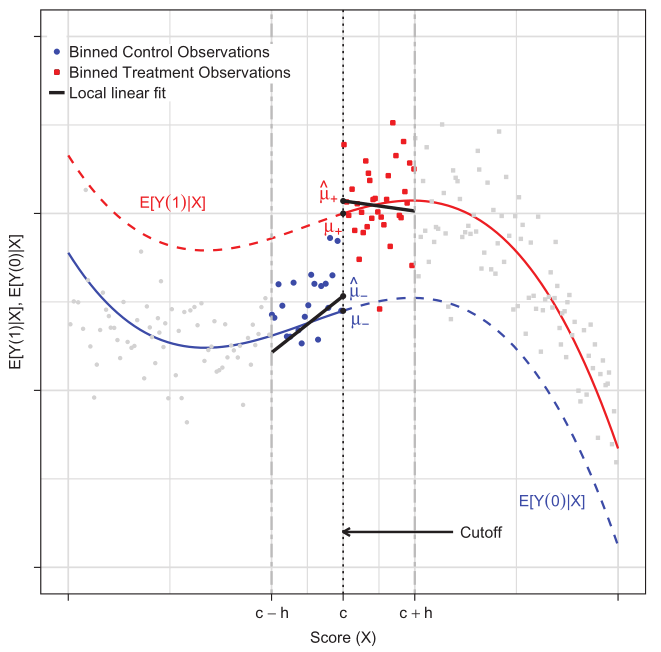
\includegraphics[scale=0.35]{../04-figures/07/06.PNG}
			\caption{\cite{cattaneo_practical_2019}}
		\end{figure}
	\end{column}
\end{columns}

\end{frame}


\begin{frame}
\frametitle{Kernel function}

\begin{columns}
	\begin{column}{0.3\textwidth}
	  \footnotesize
		Triangular is typically default.\bigskip
		
		In practice, does not make a big difference.
	\end{column}
	\begin{column}{0.7\textwidth}
		\begin{figure}
			\centering
			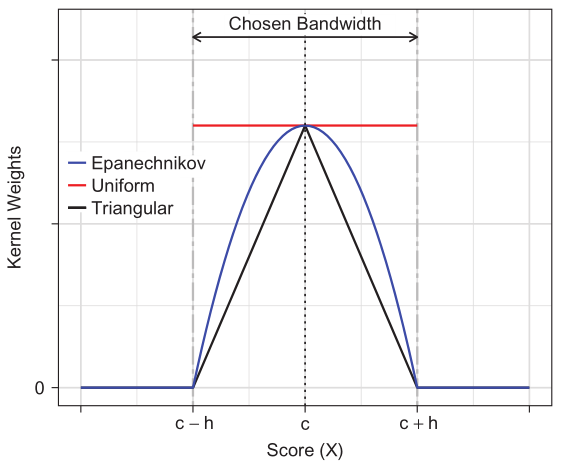
\includegraphics[scale=0.5]{../04-figures/07/07.PNG}
			\caption{\cite{cattaneo_practical_2019}}
		\end{figure}
	\end{column}
\end{columns}

\end{frame}


\begin{frame}
\frametitle{Polynomial order}

First order: $Y_i = \beta_0 + \beta_1X + \epsilon_i$.

Second order: $Y_i = \beta_0 + \beta_1X + \beta_2X^2 + \epsilon_i$.\bigskip
\pause

The default tends to be the linear RD estimator (first order).

\end{frame}



\begin{frame}
\frametitle{Bandwidth selection}
Very consequential for estimation.\bigskip
\pause

Accuracy of approximation can be improved by reducing bandwidth.\bigskip
\pause

The downside is that variance of estimator increases because fewer observations make it in.\bigskip
\pause

``Bias-variance tradeoff'' in bandwidth choice.

\end{frame}


\begin{frame}
\frametitle{Bandwidth selection}

\begin{figure}
\centering
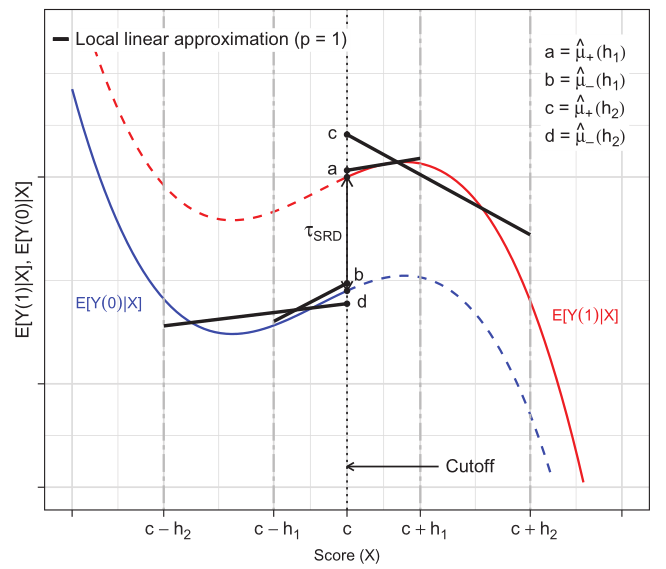
\includegraphics[scale=0.35]{../04-figures/07/08.PNG}
\caption{\cite{cattaneo_practical_2019}}
\end{figure}

Software will handle this automatically.
\end{frame}


\subsection{Choices in estimation}
\begin{frame}
\frametitle{Regression: linear model \& common slope}
Assumptions:

\begin{itemize}
\item linearity: $E[Y_{0i} | X_i = x]$ and $E[Y_{1i} | X_i = x]$ are linear in $x$
\item constant treatment effect ($\tau$)
\end{itemize}\bigskip
\pause

Implication:

\begin{equation}
\begin{cases}
E[Y_{0i} | X_i] = \beta_0 + \beta_1*X_i \\
E[Y_{1i} | X_i] = \beta_0 + \tau + \beta_1*X_i
\end{cases}
\end{equation}

\end{frame}

\begin{frame}
\frametitle{Regression: linear model \& common slope}



\begin{figure}
\centering
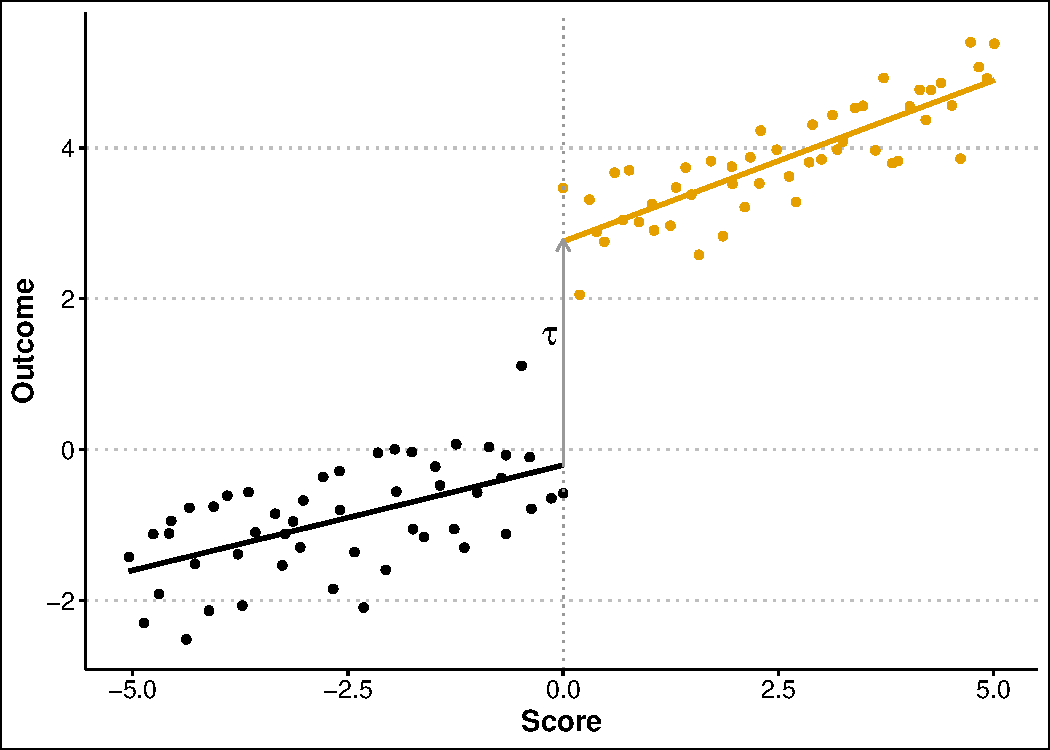
\includegraphics[scale=0.4]{../04-figures/07/09.pdf}
\caption{Model is $Y_i = \beta_0 + \tau D_i + \beta_1X_i + \epsilon_i$}
\end{figure}

Use transformed version of $X$: deviation from $c$.
\end{frame}


\begin{frame}
\frametitle{Regression: linear model \& different slope}
Assumptions:

\begin{itemize}
\item linearity: $E[Y_{0i} | X_i = x]$ and $E[Y_{1i} | X_i = x]$ are linear in $x$
\item varying treatment effect ($\tau$) along $X$
\end{itemize}\bigskip
\pause

Implication:

\begin{equation}
\begin{cases}
E[Y_{0i} | X_i] = \beta_0 + \beta_1*X_i \\
E[Y_{1i} | X_i] = \beta_0 + \tau + (\beta_1 + \phi)*X_i
\end{cases}
\end{equation}

$\phi$ can be either positive or negative.

\end{frame}


\begin{frame}
\frametitle{Regression: linear model \& different slope}



\begin{figure}
\centering
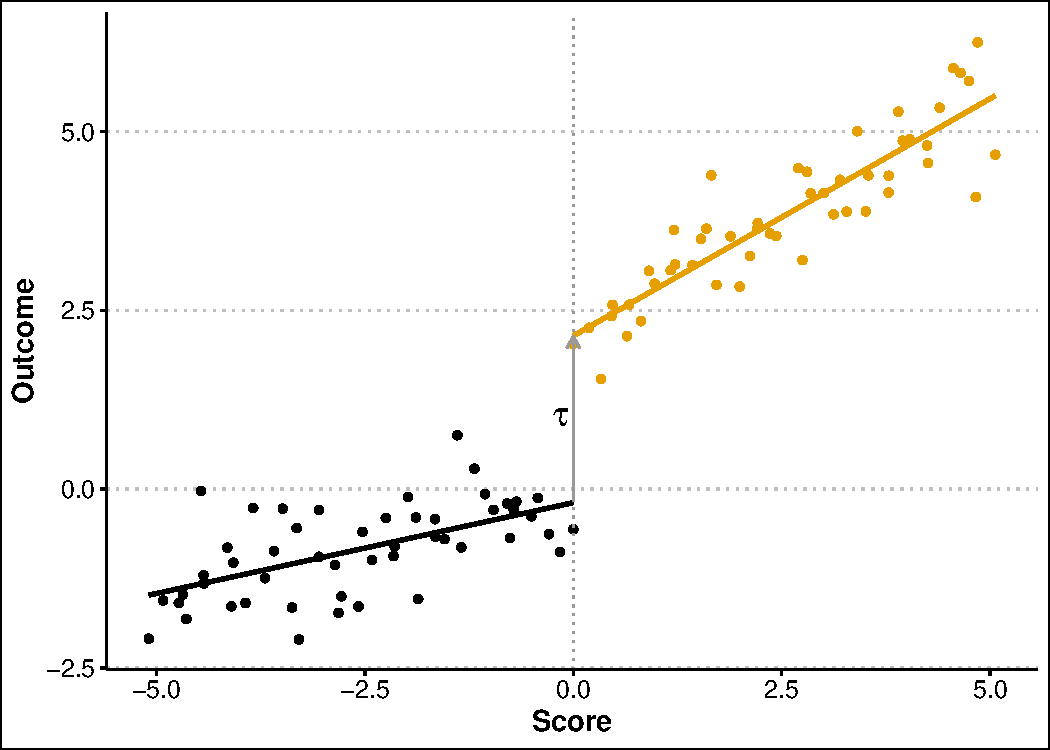
\includegraphics[scale=0.4]{../04-figures/07/10.pdf}
\caption{Model is $Y_i = \beta_0 + \tau D_i + \beta_1X_i + \phi D_iX_i + \epsilon_i$}
\end{figure}

Use transformed version of $X$: deviation from $c$.
\end{frame}


\begin{frame}
\frametitle{Regression: nonlinear model}
Assumptions:

\begin{itemize}
\item non-linearity: $E[Y_{0i} | X_i = x]$ and $E[Y_{1i} | X_i = x]$ are non-linear in $x$
\item varying treatment effect ($\tau$) along $X$
\end{itemize}\bigskip
\pause

Include quadratic version of score, $X_i^2$, and interaction with $D_i$, but venture further very carefully \cite{gelman_why_2019}.\bigskip
\pause

Model: $Y_i = \beta_0 + \tau D_i + \beta_1X_i + \beta_2X^2_i + \beta_3X_iD_i + \beta_4X^2_iD_i + \epsilon_i$

\end{frame}


\section{Empirics II}

\begin{frame}[fragile]
\frametitle{\citeA{meyersson_islamic_2014} data}

What effect does political control by Islamist parties have on the political empowerment of women?\bigskip
\pause

\begin{knitrout}\footnotesize
\definecolor{shadecolor}{rgb}{0.969, 0.969, 0.969}\color{fgcolor}\begin{kframe}
\begin{alltt}
\hlstd{df_rdd} \hlkwb{<-} \hlstd{df_rdd} \hlopt
  \hlkwd{mutate}\hlstd{(}\hlkwc{iwm94} \hlstd{= iwm94} \hlopt{*} \hlnum{100}\hlstd{,}
         \hlkwc{hischshr1520f} \hlstd{= hischshr1520f} \hlopt{*} \hlnum{100}\hlstd{)}

\hlstd{out} \hlkwb{<-} \hlkwd{rdrobust}\hlstd{(df_rdd}\hlopt{$}\hlstd{hischshr1520f,}
                \hlstd{df_rdd}\hlopt{$}\hlstd{iwm94,}
                \hlkwc{kernel} \hlstd{=} \hlstr{"triangular"}\hlstd{,}
                \hlkwc{p} \hlstd{=} \hlnum{1}\hlstd{,}
                \hlkwc{bwselect} \hlstd{=} \hlstr{"mserd"}\hlstd{)}
\end{alltt}
\end{kframe}
\end{knitrout}
\end{frame}

\begin{frame}[fragile]
\frametitle{Effect of Islamic party power}

\begin{knitrout}\tiny
\definecolor{shadecolor}{rgb}{0.969, 0.969, 0.969}\color{fgcolor}\begin{kframe}
\begin{alltt}
\hlkwd{summary}\hlstd{(out)}
\end{alltt}
\begin{verbatim}
Sharp RD estimates using local polynomial regression.

Number of Obs.                 2630
BW type                       mserd
Kernel                   Triangular
VCE method                       NN

Number of Obs.                 2315          315
Eff. Number of Obs.             529          266
Order est. (p)                    1            1
Order bias  (q)                   2            2
BW est. (h)                  17.243       17.243
BW bias (b)                  28.575       28.575
rho (h/b)                     0.603        0.603
Unique Obs.                    2313          315

=============================================================================
        Method     Coef. Std. Err.         z     P>|z|      [ 95% C.I. ]       
=============================================================================
  Conventional     3.020     1.427     2.116     0.034     [0.223 , 5.816]     
        Robust         -         -     1.776     0.076    [-0.309 , 6.276]     
=============================================================================
\end{verbatim}
\end{kframe}
\end{knitrout}
\end{frame}


\begin{frame}[fragile]
\frametitle{Effect of Islamic party power}



\begin{figure}
\centering
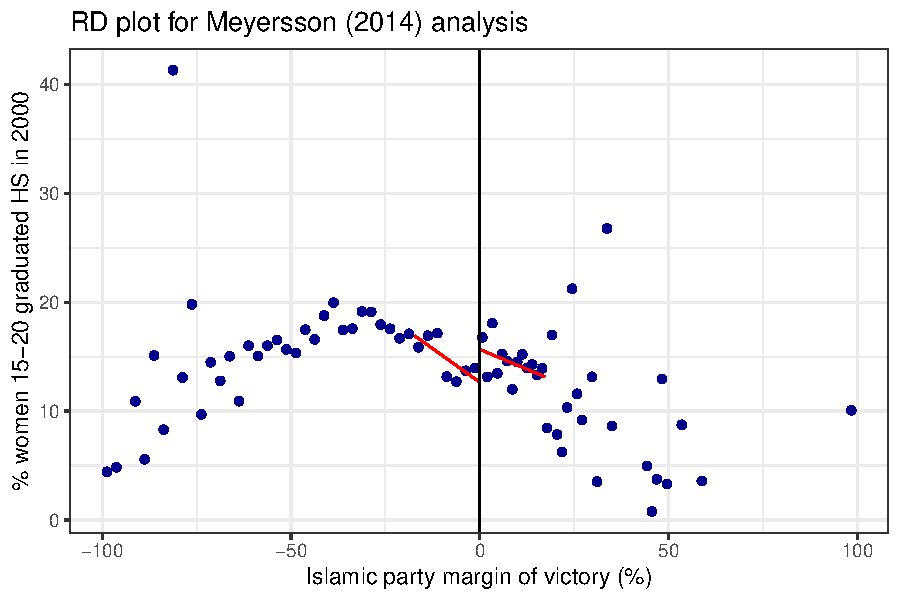
\includegraphics[scale=0.7]{../04-figures/07/11.pdf}
\end{figure}

\end{frame}


\begin{frame}
\frametitle{Alternative specifications}

\begin{figure}
\centering
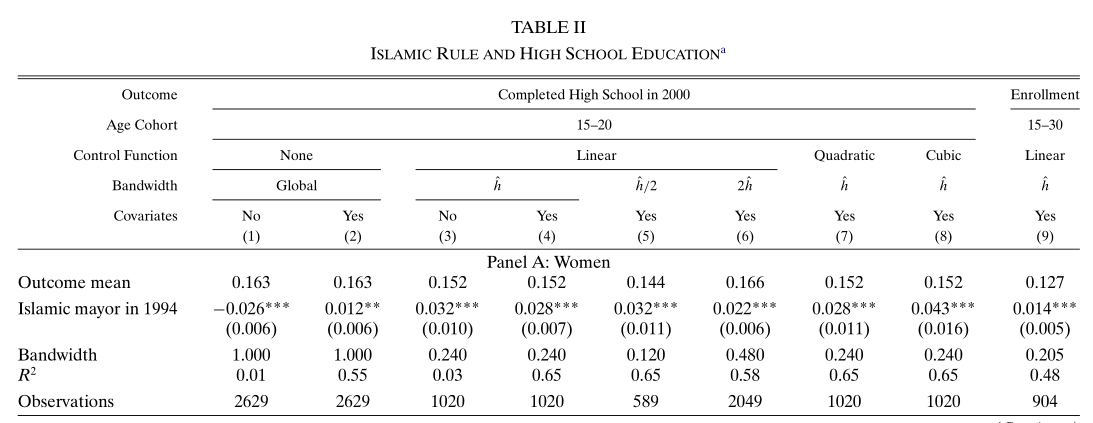
\includegraphics[scale=0.4]{../04-figures/07/12.PNG}
\end{figure}

\end{frame}


\section{Diagnostics and Falsification Checks}

\begin{frame}
\frametitle{Diagnosing an RD design}
Treatment assignment mechanism is known to researcher, and based on observable features.\bigskip
\pause

A whole array of approaches!

\begin{itemize}
\item null effect on pre-treatment covariates and placebo outcomes
\item score density continuity around cutoff
\item treatment effect at artificial cutoff values
\item excluding observations near cutoff
\item sensitivity to bandwidth choices
\end{itemize}

\end{frame}


\begin{frame}
\frametitle{Pre-treatment covariates and placebos}
Are treatment and control units similar around the cutoff on observables?\bigskip
\pause

Two types:

\begin{itemize}
\item \textcolor{orange}{pre-treatment covariates}: determined before assignment to treatment;
\item \textcolor{orange}{placebo outcomes}: post-treatment, but not affected by treatment.
\end{itemize}

\end{frame}


\begin{frame}
\frametitle{Pre-treatment covariates: \citeA{meyersson_islamic_2014}}

\begin{figure}
\centering
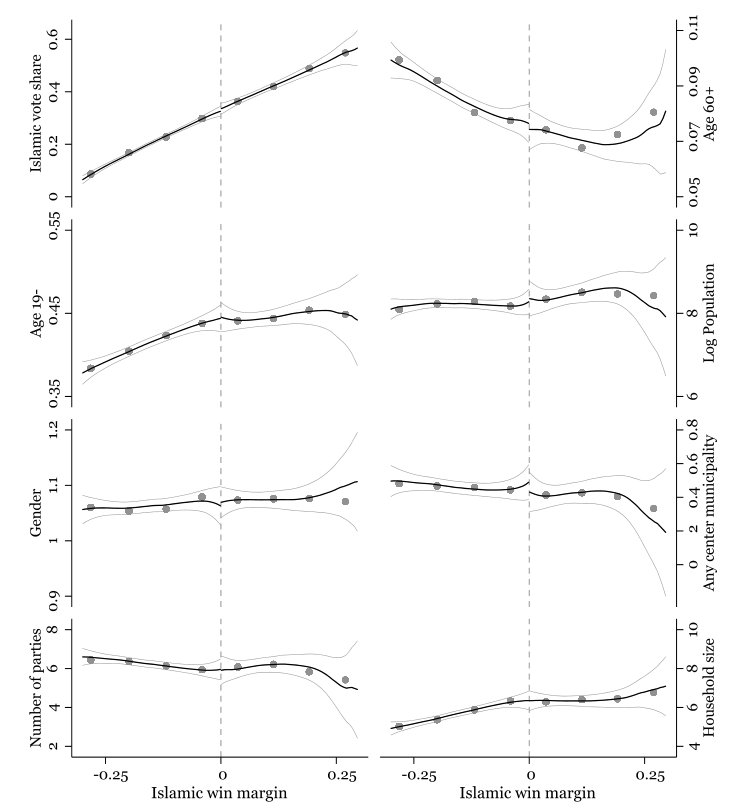
\includegraphics[scale=0.3]{../04-figures/07/13.PNG}
\end{figure}

\end{frame}


\begin{frame}
\frametitle{Score density}
Is number of observations different below and above the cutoff? (if local randomization holds, it shouldn't be)\bigskip
\pause

Could indicate active manipulation of score (e.g. contesting test results below passing threshold).\bigskip
\pause

Easily done with a density test, to test for sorting.

\end{frame}


\begin{frame}
\frametitle{Score density: \citeA{meyersson_islamic_2014}}

\begin{figure}
\centering
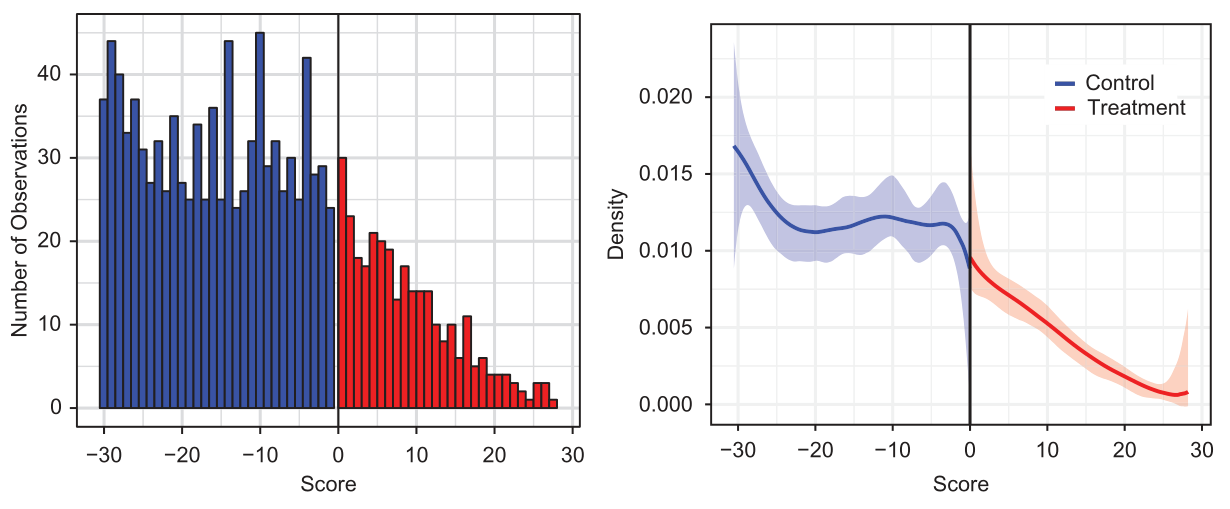
\includegraphics[scale=0.35]{../04-figures/07/14.PNG}
\caption{\cite{cattaneo_practical_2019}}
\end{figure}

\end{frame}


\begin{frame}
\frametitle{Artificial cutoff values}
\textcolor{orange}{Key} identifying assumption: continuity of regression function at cutoff in the absence of treatment.\bigskip
\pause

Impossible to test at cutoff, but the opposite can be tested outside of it.\bigskip

Are there discontinuities in regression functions away from cutoff which can't be explained?

\end{frame}


\begin{frame}
\frametitle{Artificial cutoff values: \citeA{meyersson_islamic_2014}}

\begin{figure}
\centering
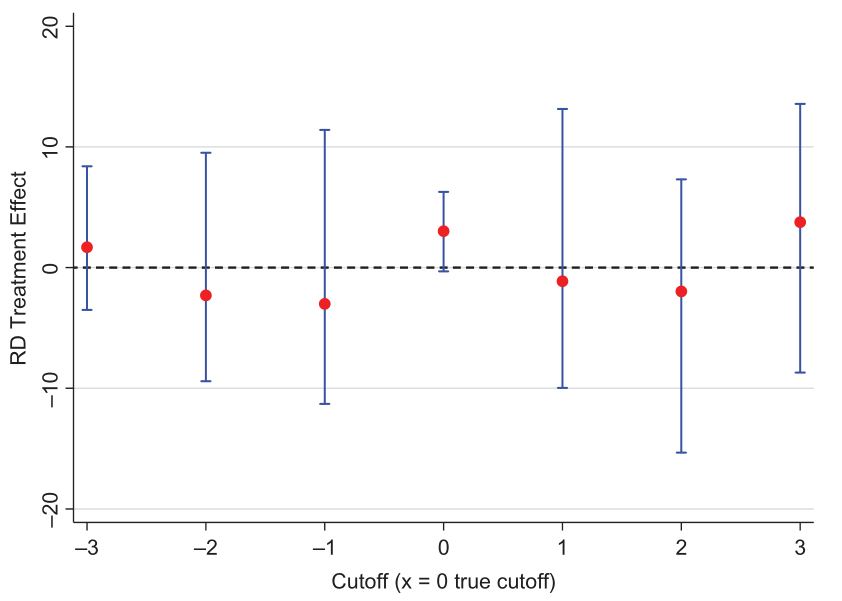
\includegraphics[scale=0.3]{../04-figures/07/15.PNG}
\caption{\cite{cattaneo_practical_2019}}
\end{figure}

No evidence of discontinuous jump at artificial cutoffs.

\end{frame}



\begin{frame}
\frametitle{Sensitivity to cases near cutoff}
Are results sensitive to excluding cases near the cutoff?\bigskip
\pause

If any score manipulation took place, these would be the most likely units to engage in this.\bigskip
\pause

Gradually remove observations in a window around the cutoff, $[c-w; c+w]$, and re-run analysis.

\end{frame}


\begin{frame}
\frametitle{Sensitivity to cases near cutoff: \citeA{meyersson_islamic_2014}}

\begin{figure}
\centering
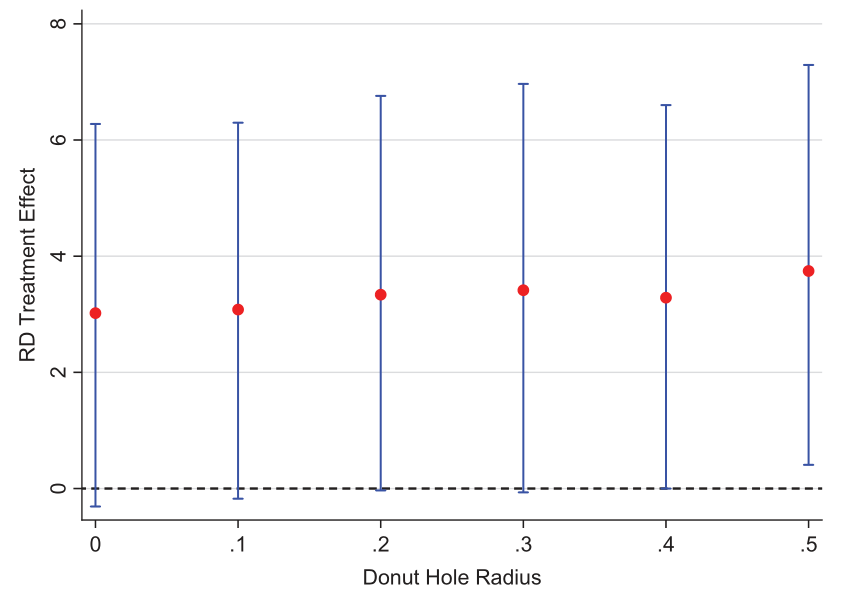
\includegraphics[scale=0.35]{../04-figures/07/16.PNG}
\caption{\cite{cattaneo_practical_2019}}
\end{figure}

\end{frame}


\begin{frame}
\frametitle{Sensitivity to bandwidth choice: \citeA{meyersson_islamic_2014}}

\begin{figure}
\centering
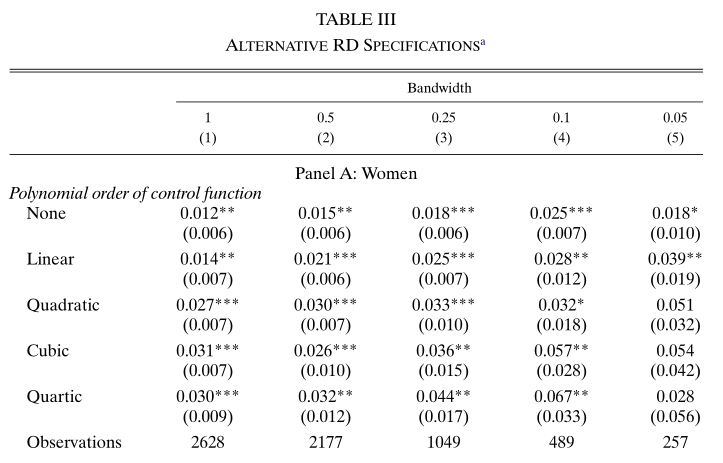
\includegraphics[scale=0.4]{../04-figures/07/17.PNG}
\end{figure}

In this instance, results are largely insensitive to bandwidth.

\end{frame}


\section{Fuzzy RD}

\begin{frame}
\frametitle{Fuzzy RD: features}

In sharp RD we assumed:

\begin{itemize}
\item all units assigned to treatment actually take it
\item no units assigned to control take treatment
\end{itemize}\bigskip
\pause

In fuzzy RD, those assumptions are no longer met:

\begin{itemize}
\item some units assigned to treatment fail to receive it
\item some control units manage to get treatment
\end{itemize}

\end{frame}


\begin{frame}
\frametitle{Fuzzy RD: features}

Probability of \textit{receiving} treatment still jumps at cutoff, but is no longer either 0 or 1.\bigskip
\pause

$T_i$: treatment assignment.

$D_i$: treatment take-up.\bigskip
\pause

For some units $T_i \neq D_i$.

\end{frame}


\begin{frame}
\frametitle{Fuzzy RD: features}

\begin{figure}
\centering
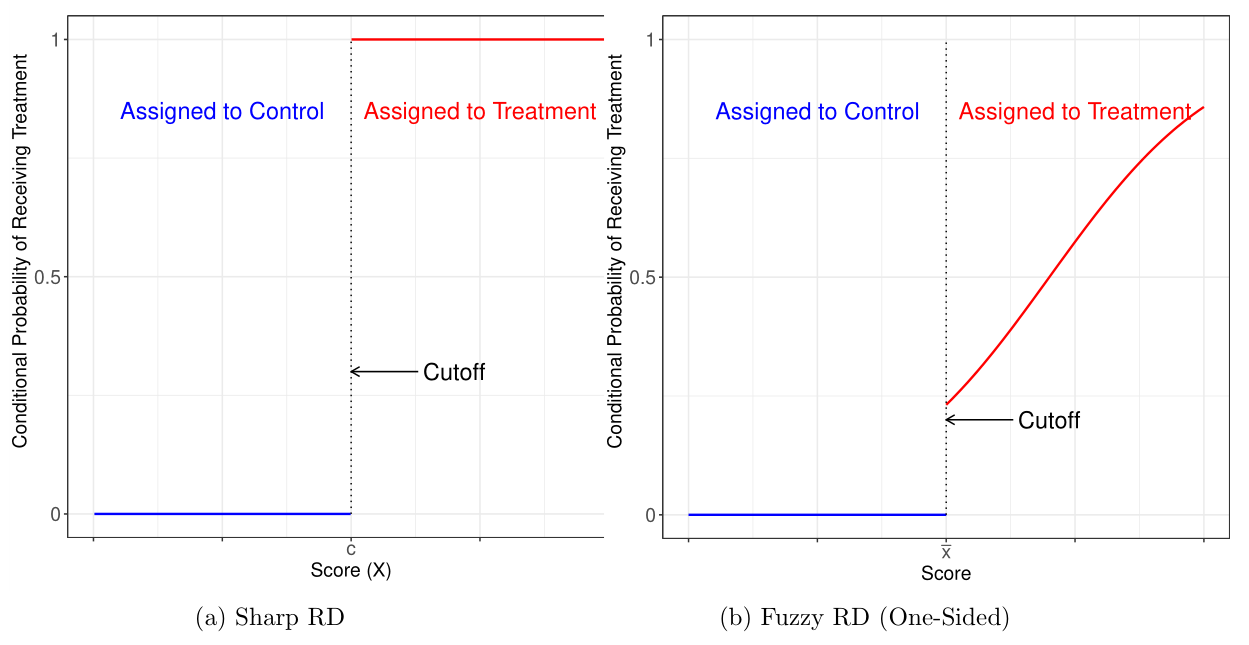
\includegraphics[scale=0.4]{../04-figures/07/18.PNG}
\end{figure}

Treatment taken: $D_i = T_iD_{1i} + (1 - T_i)D_{0i}$.

\end{frame}


\begin{frame}
\frametitle{IV similarity}
Similarity to IV: $T_i$ only impacts $Y_i$ through its effect on $D_i$ (\textit{exclusion restriction}).\bigskip
\pause

Interest is in both effect of $T_i$ (which is a standard sharp RD estimation), and of $D_i$.\bigskip
\pause

Can be estimated using either the continuity-based approach or the local randomization one.

\end{frame}


\begin{frame}
\frametitle{Estimation: continuity-based}
Effect of $T_i$ is clear, as compliance with the assignment rule is perfect (unlike take-up).\pause

\begin{align*}
\tau_{ITT} &= \lim_{x \downarrow c}E[Y_i | X_i = x] - \lim_{x \uparrow c}E[Y_i | X_i = x] = \\
           &= E[(D_{1i} - D_{0i})(Y_{1i} - Y_{0i}) | X_i = c]
\end{align*}\pause

$\tau_{SRD} \neq \tau_{ITT}$, since the latter also includes $D_{1i} - D_{0i}$.\bigskip
\pause

With perfect compliance, $D_{1i} - D_{0i} = 1 - 0 = 1$ for all $i$.

\end{frame}


\begin{frame}
\frametitle{Estimation: continuity-based}
We can also define the \textcolor{orange}{first-stage} effect: effect (at the cutoff) of being assigned to treatment on treatment take-up.\pause

\begin{align*}
\tau_{FS} &= \lim_{x \downarrow c}E[D_i | X_i = x] - \lim_{x \uparrow c}E[D_i | X_i = x] = \\
          &= E[D_{1i} - D_{0i} | X_i = c]
\end{align*}\pause

Both $\tau_{ITT}$ and $\tau_{FS}$ are sharp RD parameters, and can be estimated as we saw above.

\end{frame}


\begin{frame}
\frametitle{Estimation: treatment effect}
Additional assumption: \textcolor{orange}{monotonicity}.

Unit $i$ that refuses treatment at cutoff $c_1$ must refuse it for any cutoff $c_2 > c_1$. Similarly, treatment taken at cutoff $c_1$ should also be taken at cutoff $c_2 < c_1$.\bigskip
\pause

It can be shown that under this condition (plus continuity):

\begin{equation}
\footnotesize
LATE = \tau_{FRD} = \frac{\tau_{ITT}}{\tau_{FS}} = \frac{\lim_{x \downarrow c}E[Y_i | X_i = x] - \lim_{x \uparrow c}E[Y_i | X_i = x]}{\lim_{x \downarrow c}E[D_i | X_i = x] - \lim_{x \uparrow c}E[D_i | X_i = x]}
\end{equation}

Estimation is performed with 2SLS.
\end{frame}


\section{Wrap-up}

\begin{frame}
\frametitle{Validity}
Though assignment is ``as-if-random'', it's not purposeful random assignment.\bigskip
\pause

Internal validity is good: with enough data around the cutoff, we can estimate $\tau$ at cutoff.\bigskip
\pause

External validity is less good: effect is local, at the cutoff. We cannot extrapolate to other values $X \neq c$ except by making additional assumptions.\bigskip
\pause

However, a very flexible framework: score can be categorical, multiple scores and multiple cutoffs can be accommodated. 
\end{frame}


\begin{frame}
\frametitle{Summary}
Though data-intensive, the RDD framework is very powerful.\bigskip
\pause

It comes with a host of tools for model assessment and validation.\bigskip
\pause

Can be adapted to a host of policy-relevant empirical settings: educational achievement, corruption, distributive politics, political accountability.

\end{frame}


% END
\begin{frame}
\begin{center}
    \Huge Thank \textcolor{orange}{you} for the kind attention!
\end{center}
\end{frame}

% REFERENCES %

\begin{frame}[allowframebreaks]
\bibliographystyle{apacite}
\scriptsize\bibliography{../Bibliography}
\end{frame}

\end{document}
